\section{Beam pattern to aperture conversion}

In this section the aim is to solve the equation \ref{eq:holo_nearfield}. We will separate the problem in two parts as shown in the equations \ref{eq:nearfield_reduced} and \ref{eq:fourier_like_integral}.


\begin{equation}
    \label{eq:nearfield_reduced}
    F(\xi, \eta) = \frac{i}{\lambda}\frac{e^{-ikR}}{R} exp\left(-ik[\delta p_1(\xi,\eta)+\delta p_2(\xi, \eta)]\right) \cdot \Phi(\xi, \eta)
\end{equation}
\begin{equation}
    \label{eq:fourier_like_integral}
    \begin{split}
        \Phi(\xi, \eta) = \int f(u,v)exp\left(ik(u\xi+v\eta)\right) \cdot \Biggl(1-ik\biggl[ u \frac{\xi(\xi^2+\eta^2)}{2R^2} + \\
        v \frac{\eta(\xi^2 +\eta^2)}{2R^2}-u^2\frac{\xi^2}{2R}-v^2\frac{\eta^2}{2R}-uv\frac{\xi\eta}{R} \biggr] \Biggr)
    \end{split}
\end{equation}

Since the distance of the APEX holography transmitter is at $1835m$, the first thing to investigate is if we need to solve numerically the integral shown in \ref{eq:fourier_like_integral} or if we just can take the first order approximation and compute the 2D Fourier integral using a Fast Fourier transform algorithm.


The current pipeline has the option of use both methods, but when applying them to the collected data the error atributted to the high order terms is neglectable. The figures \ref{fig:high_order_terms_power} and \ref{fig:high_order_terms_power_diff} shows the magnitude of the bona fide fourier transform and the high order integral terms in one of the APEX holography measurements. The figure \ref{fig:high_order_terms_power_diff} shows that the biggest effect of the high order terms are around the edges of the telescope, but even there the difference between the bona fide Fourier transform is $30dB$ higher than the values given by the high order integral terms.


We also had run the pipeline using the complete with and without considering the high order terms and the final difference in the RMS surface error maps is in the order of the $nm$ as its shown in the figure \ref{fig:high_fft_surf_error}


\begin{figure}
    \centering
    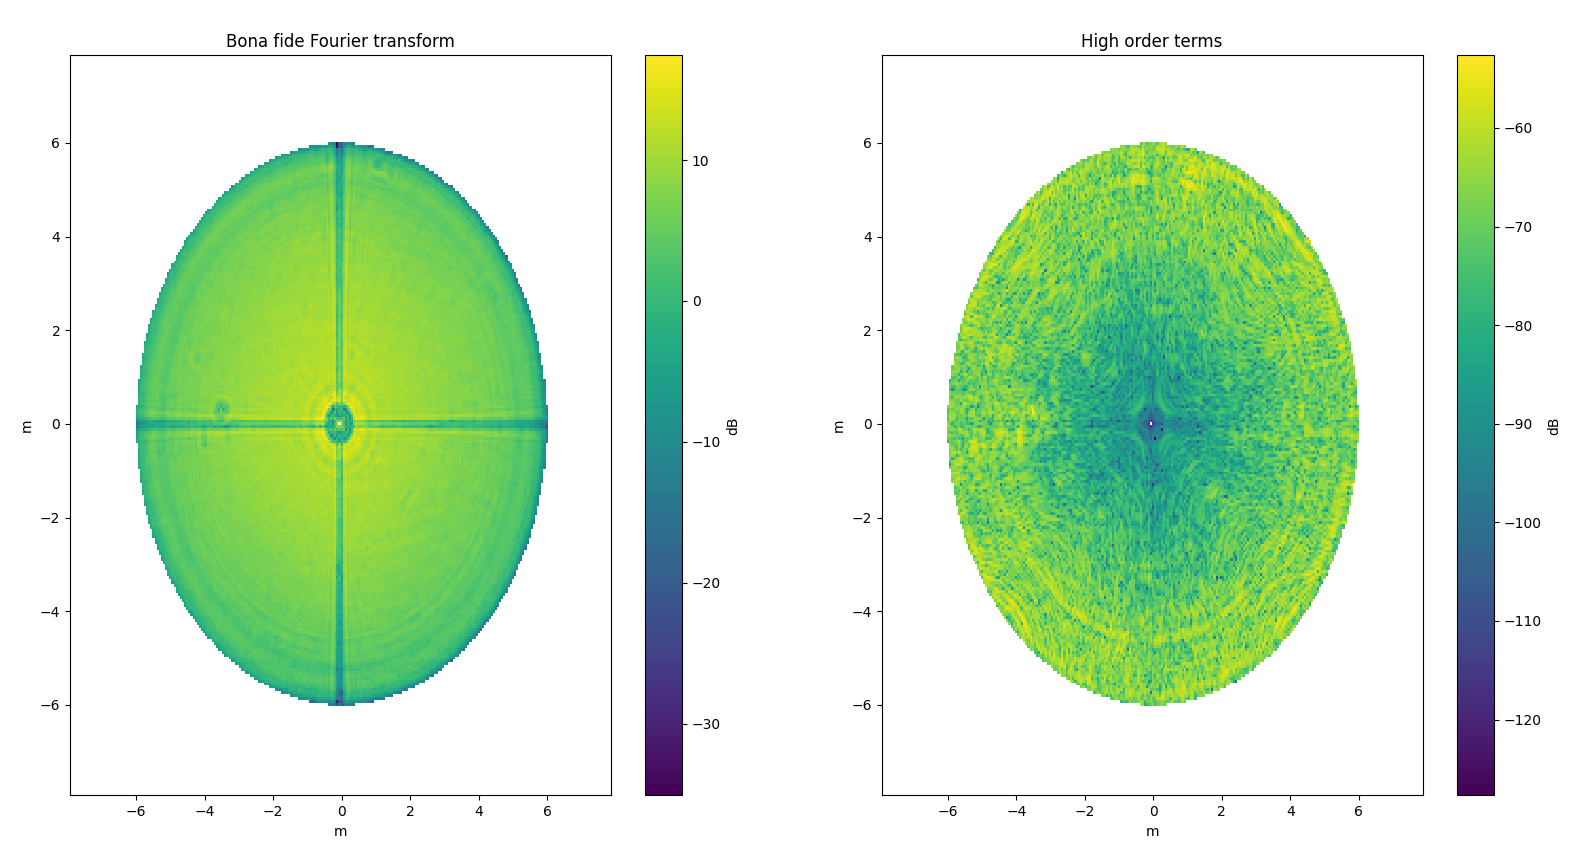
\includegraphics[width=1\textwidth]{images/high_order_fft.png}
    \caption{Power of the bona fide Fourier transform and the high order integral terms. Note that the scales are different for each map otherwise the image will be completly saturated.}
    \label{fig:high_order_terms_power}
\end{figure}


\begin{figure}
    \centering
    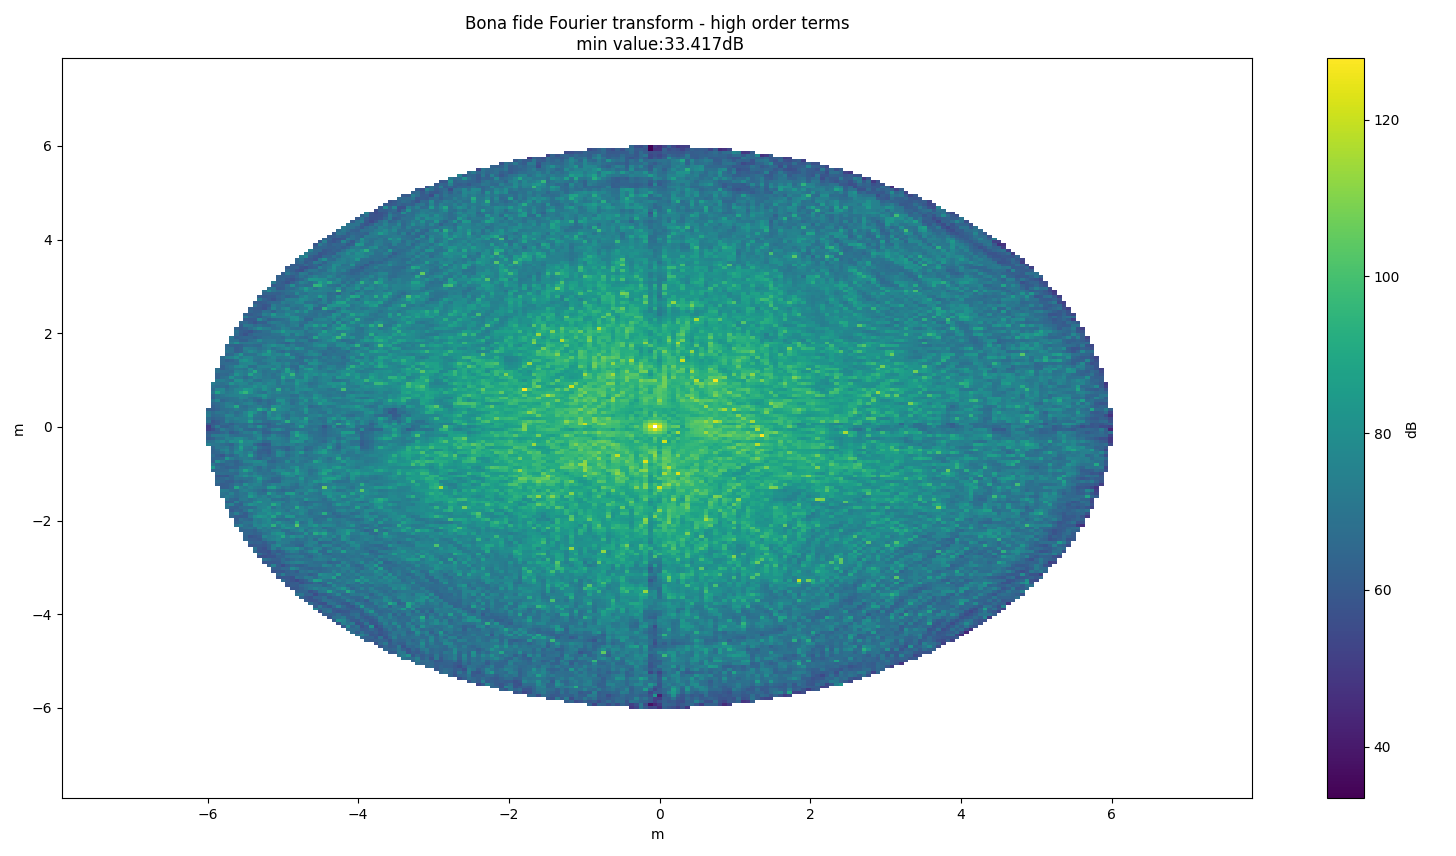
\includegraphics[width=0.9\textwidth]{images/fft_high_order_difference.png}
    \caption{Power difference of bona fide Fourier transform and the high order integral terms.}
    \label{fig:high_order_terms_power_diff}
\end{figure}


\begin{figure}
    \centering
    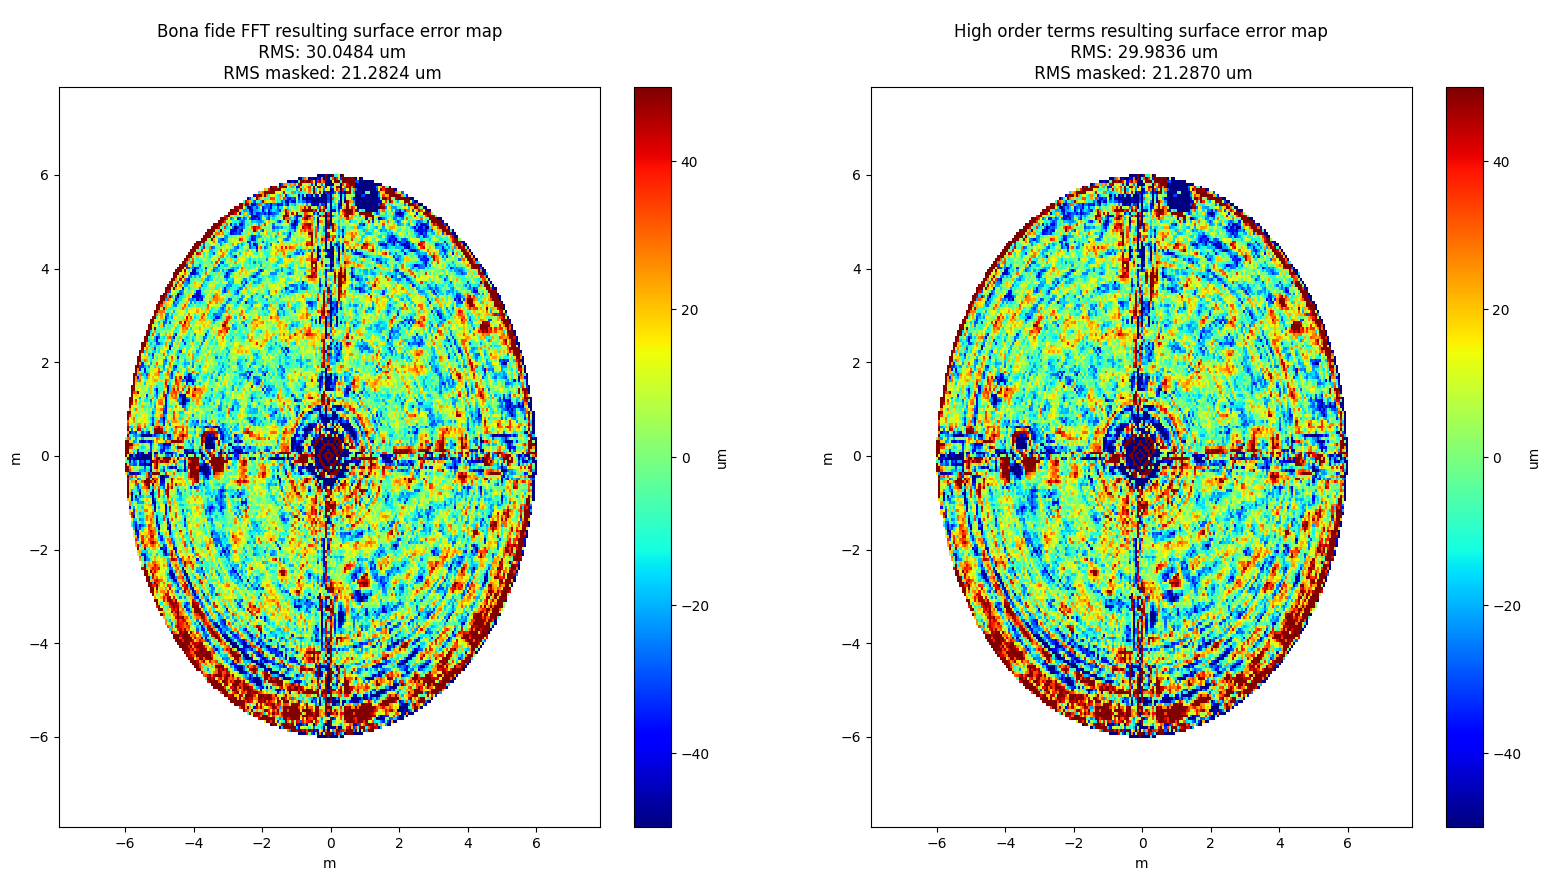
\includegraphics[width=1\textwidth]{images/high_vs_fft_surf_error.png}
    \caption{Final map given by the current pipeline considering solving the complete integral or just sticking with the Fourier transform. The final RMS difference is in the $nm$ scale.}
    \label{fig:high_fft_surf_error}
\end{figure}




\subsection{Defocus, Nearfield and tilt correction}
The defocus and nerafield corrections are contained in the $\delta p_1$ and $\delta p_2$ terms, where we need to find the proper $\delta f$ that match the measurements. Aditionally the measurement could have a tilt in the measure that needs to be removed. The tilting of a field can be generated by the equation \ref{eq:aperture_tilt}.

To find the parameters $(\delta f, \theta_x, \theta_y)$ we run an optimization process where the target is found the parameters that minimize the RMS surface error.

\begin{equation}
    E_{tilted}(x,y) = E(x,y)\exp\left(\frac{2\pi}{k}i\left(\theta_x\cdot x+ \theta_y \cdot y\right)\right)
    \label{eq:aperture_tilt}
\end{equation}


The figure \ref{fig:nearfield_correction} shows an example of the before and after of the corrections.



\begin{figure}
    \centering
    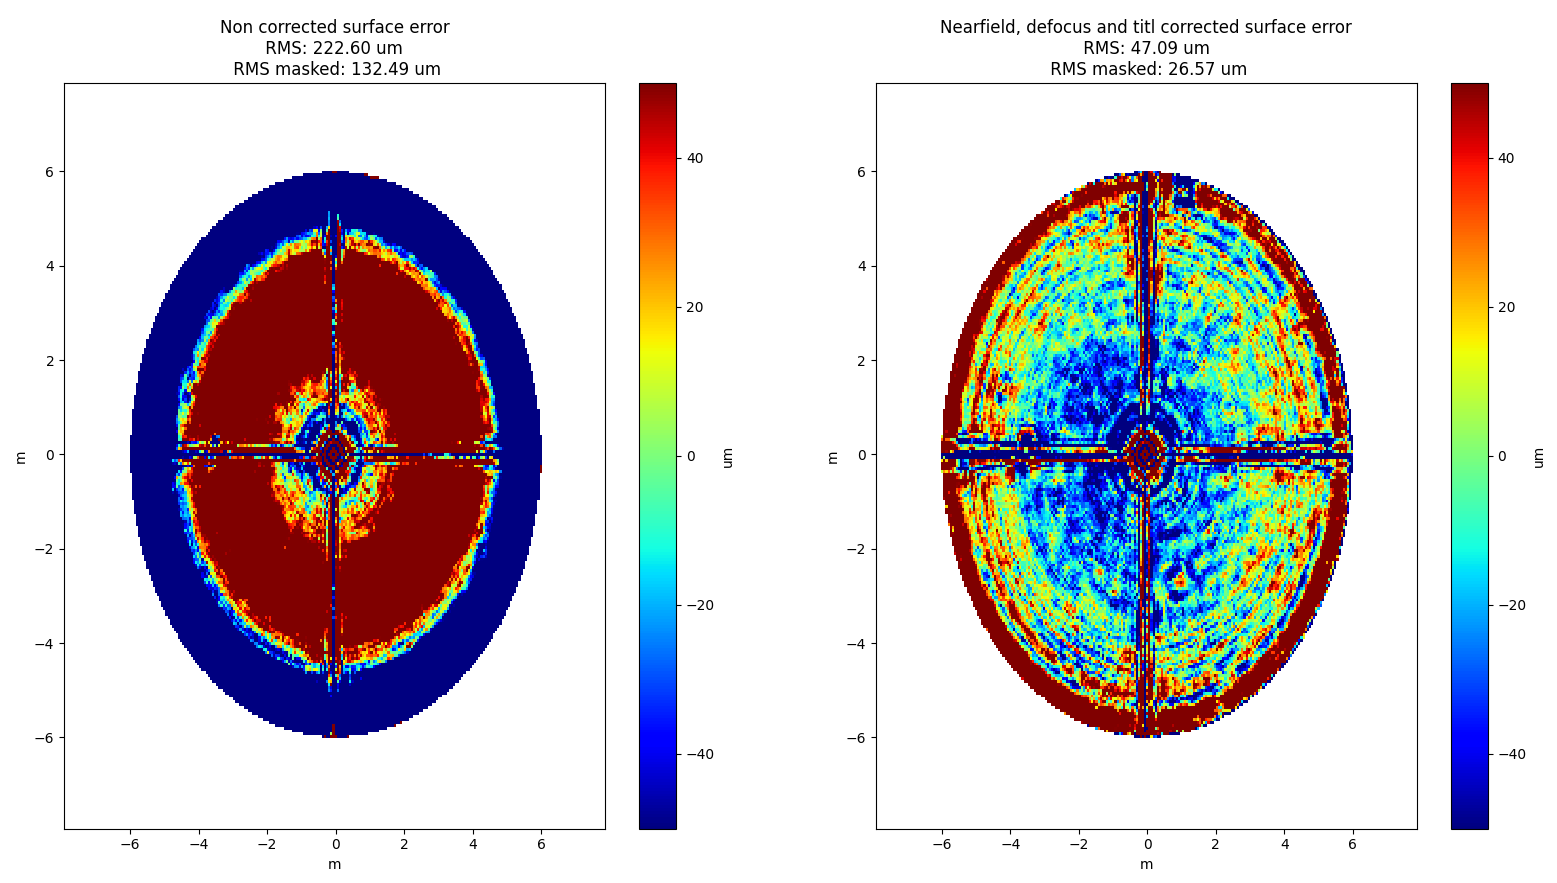
\includegraphics[width=1\textwidth]{images/nearfield_correction.png}
    \caption{Defocus, nearfield and tilt corrections. For this map the defocus and tilt values found by the optimization process were $\delta f = -15.36mm$, $\theta_x=-1.36arcsec$, $\theta_y =-1.41arcsec$}.
    \label{fig:nearfield_correction}
\end{figure}







